\section{Preliminaries}\label{sec:prelim}



%We fix in the rest of the paper an alphabet $\Sigma$ which is a ranked set whose elements, called letters, are either . We let  $\Sigma_1$ and $\Sigma_2$ be the set of \emph{unary} and \emph{binary} letters of $\Sigma$ respectively.  
 %\todo{Les transformer en $\Sigma$?}
 
\subsection{Tree-width 2 graphs}

\begin{definition}[Ranked sets]
A \emph{ranked set} is a set where every element has an associated \emph{arity} in $\mathbb{N}$. Elements of arity $0$ are called \emph{nullary}, of arity $1$ are called \emph{unary}, of arity $2$ are called \emph{binary} etc. An \emph{arity-preserving function} is a function between two ranked sets which does not change arities.
\end{definition}

We fix in the rest of the paper an alphabet $\Sigma$, which is a ranked set whose \emph{letters} are either unary or binary. We denote their sets $\Sigma_1$ and $\Sigma_2$ respectively.

\begin{definition}[Graphs]
 A graph consists of:
\begin{itemize}
\item a (not ranked) set $V$ of \emph{vertices},
\item a ranked set $E$ of \emph{edges} of arity $1$ or $2$,
\item a function $E\mapsto V^*$ which maps each $n$-ary edge to its \emph{interface}, which has length $n$,
\item an arity-preserving \emph{labeling} $E\mapsto \Sigma$,
\item a list of size $n\in\set{1,2}$ called its \emph{interface}. The number $n$ is called the arity of the \emph{graph}.
\end{itemize} \todo{define subgraph}

The first element of the interface of an edge is called its \emph{source}, and the last element is called its \emph{target}.
The first element of the interface of a graph  is called its \emph{input}, and the last element is called its \emph{output}\footnote{For unary graphs and edges, the input equals the output.}. All the vertices of a graph which are not in the interface are called \emph{inner vertices}. An \emph{$a$-edge} is an edge labeled by the letter $a$.
 
 A  graph is \emph{empty} if it has no edges, and if all its vertices are interface vertices.  
 
 If $v, w$ are two vertices of a graph $G$, we denote by $(v,G,w)$ the graph obtained from $G$ by declaring $v$ as its input and $w$ as its output.
\end{definition}



%\begin{definition}[Graphs] 
% A \emph{graph} $G$ is  a tuple $(V,E_1,E_2, s, t, l_1, l_2, \iota, o)$, where $V$ is a set of \emph{vertices}, $E_1$ and $E_2$ are two disjoint sets  of \emph{unary} and \emph{binary edges}, $s:E_1\uplus E_2\to V$  and $t:E_2\to V$ are a \emph{source} and a \emph{target} functions specifying the source and the target of each edge\footnote{For unary edges, we specify only their source.}, $l_1:E_1\to \Sigma_1$ and $l_2:E_2\to \Sigma_2$ are \emph{labeling functions}  indicating the label of each edge,  $\iota$ is the  \emph{input} vertex and $o$ is the \emph{output} vertex, $\iota$ and $o$ are the \emph{interface vertices} of $G$. All the vertices of $G$ which are not interface vertices are called \emph{inner vertices}. The \emph{interface of $G$} is the pair $(\iota, o)$ if $\iota\neq o$, or the vertex $\iota$ otherwise.   An \emph{$a$-edge} is an edge labeled by the letter $a$. We say that $G$ is \emph{unary} if $\iota=o$, and \emph{binary} otherwise. The \emph{interface} of a binary edge $e$ is $(s(e),t(e))$, the interface of a unary edge $e$ is $s(e)$. An \emph{interface in} $G$ is a list of vertices of length $1$ or $2$. A  graph is \emph{empty} if it has no edges, and if all its vertices are interface vertices.  
%  %\todo{Do it use it?} \todo{define interface in a graph and its arity}
% \end{definition}
   \begin{remark} What we call here a graph is what is usually called a hypergraph (because of the unary edges) with interface. 
   \end{remark}

   %\todo{The way we depict graphs, forget the orientation of letters.}
\begin{example}\label{ex:graphs}  We depict graphs  with unlabeled ingoing and outgoing arrows to denote the input and the output, respectively.  The $c$-edge in the leftmost graph below is a unary edge.   The graph in the middle is a unary graph.
 \begin{center}
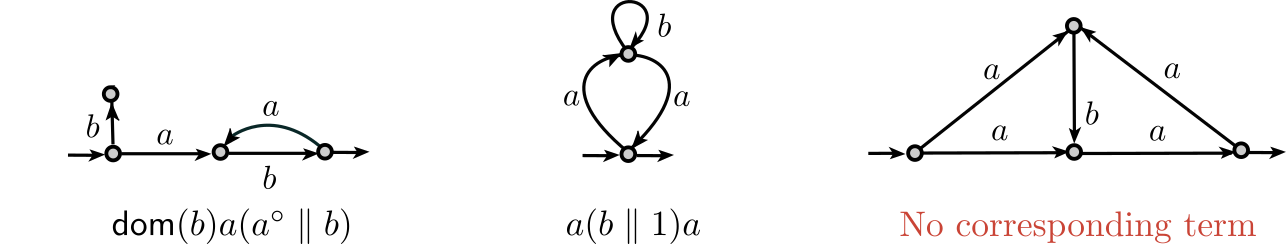
\includegraphics[scale=.35]{Pictures/example-graph}
 \end{center}
 \end{example}


  
\begin{definition}[$\TWT$ graphs]\label{def:graph-terms}
Consider the  \emph{signature $\sigma$} which is a ranked set containing the binary operations $\cdot$ and $\parallel$, the unary operations ${\ }^\circ$ and $\dom$, and the nullary operations $1$ and $\top$. We define \emph{$\TWT$ terms} as the terms generated by the signature $\sigma$ and the alphabet $\Sigma$: 
\begin{align*}
t,u:=\  a\ \mid\ t\comp u\ \mid\ (t\parallel u)\ \mid \ t^\circ\ \mid\ \dom(t)\ \mid\ 1\ \mid \ \top \qquad \qquad a\in \Sigma
\end{align*}
We define by induction the graph $\G(t)$ of a term $t$, by letting:  $$\begin{array}{l}
    
      \Gr 1=
               \begin{tikzpicture}[baseline=(0.south),xscale=.7]
                 \position (0) (0,0);
                           \initst (0); \fnst (0);
               \end{tikzpicture} \qquad
               \quad
                \Gr \top= 
               \begin{tikzpicture}[baseline=(0.south),xscale=.7]
                 \position (0) (0,0);
                 \position (1) (1,0);
                 \initst (0); \fnst (1);
               \end{tikzpicture}
           \qquad  \quad 
                \Gr a =  
              
\includegraphics[scale=1]{Pictures/unary-letter}
               \qquad
                  \quad         
                \Gr b= 
               \begin{tikzpicture}[baseline=(0.south),xscale=.7]
                 \position (0) (0,0);
                 \position (1) (1,0);
                 \initst (0); \fnst (1);
                 \edge[above] (0)(1)[b];
               \end{tikzpicture}
               \end{array} 
$$
for every $a\in \Sigma_1$ and $b\in\Sigma_2$ and interpreting the operations of the syntax as follows:
$$\begin{array}{llllll}
 G\comp H&= &  \begin{tikzpicture}[baseline=(0.south),xscale=.7]
                  \position (0) (0,0);
                  \position (1) (1.5,0);
                  \position (2) (3,0);
                  \initst (0); \fnst (2);
                  \draw[arc] (0) 
                  to node[midway,fill=white,inner sep = 0] {$G$} (1);
                  \draw[arc] (1)
                  to node[midway,fill=white,inner sep = 0] {$H$} (2);
                \end{tikzpicture} 
                &\qquad\quad G\parll  H & =  & \begin{tikzpicture}[baseline=(0.south),xscale=.7]
                 \position (0) (0,0);
                 \position (1) (1.5,0);
                 \initst (0); \fnst (1);
                 \draw[arc] (0) to[bend left] 
                 node[midway,fill=white,inner sep = 0] {$G$} (1);
                 \draw[arc] (0) to[bend right]
                 node[midway,fill=white,inner sep = 0] {$H$} (1);
               \end{tikzpicture} \\[4pt]
               \dom(G)&= &
             
\includegraphics[scale=1]{Pictures/dom}  & \qquad\quad
                   G^\circ &= &
               \begin{tikzpicture}[baseline=(0.south),xscale=.7]
                 \position (0) (0,0);
                 \position (1) (1.5,0);
                 \initst (0); \fnst (1);
                 \draw[arc] (1)  
                 to node[midway,fill=white,inner sep = 0] {$G$} (0);
               
               \end{tikzpicture}  
  
\end{array} 
$$\todo{describe more precisely}
In the picture above, we represent the graph $G$ by an arrow from its input to its output, which might be equal. For example, the graph $\dom(G)$ is obtained from $G$ by relocating the output to the input.  We usually write $tu$ instead of $t\comp u$ and give priorities to the symbols of $\sigma$ so that $ab\parll c$ parses to $(a\comp b)\parll c$.
We define the set of \emph{$\TWT$ graphs} as the graphs of the terms above. The graphs of $a$ and $a\parallel 1$, where $a\in \Sigma$, are called \emph{atomic}.
\end{definition}
We will sometimes identify terms with the graphs they generate. For example we may say that $(a\parallel b)$ is binary or connected to say that its graph is so.  

\begin{example} Below, from left to right, two $\TWT$ graphs and a graph which is not $\TWT$. 
\begin{center}
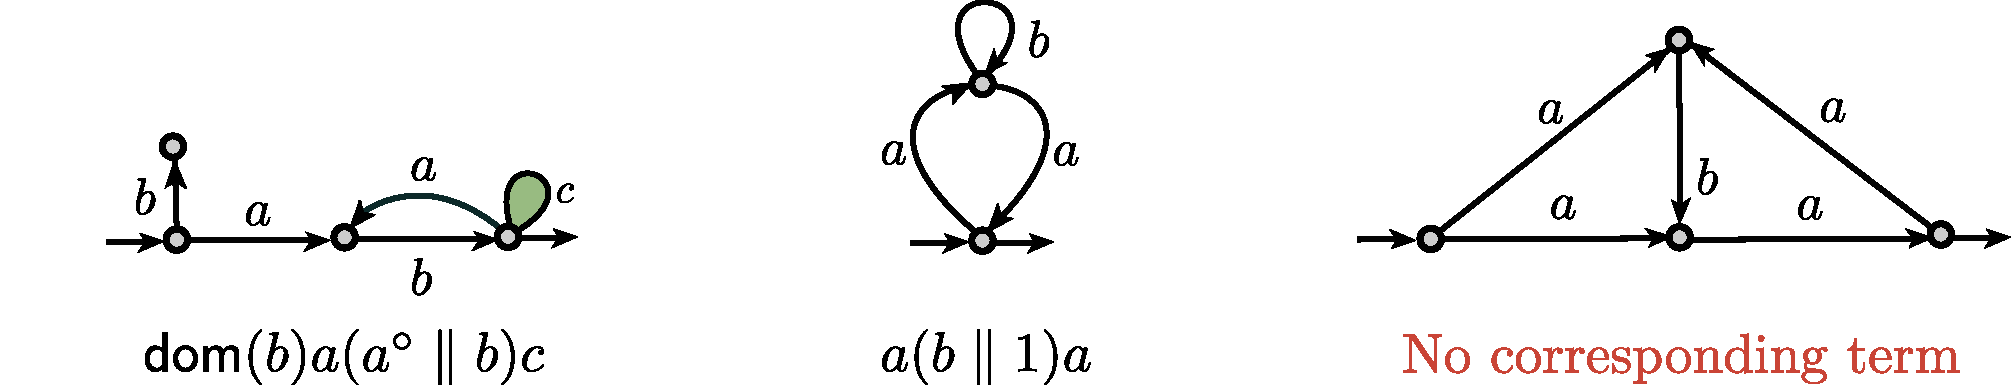
\includegraphics[scale=.35]{Pictures/example-graph-term}
\end{center}
\end{example}
%\begin{figure}
%
%\caption{Graph operations. \label{fig:graph-op}}
%\end{figure}
\begin{remark}
 The $\TWT$ graphs are exactly those graphs whose skeleton\footnote{The skeleton of a graph is the graph obtained by forgetting the labels and the orientation of the edges, and by adding an edge between the input and the output.} has tree-width 2~\cite{Cosme-LlopezP17}. 
\end{remark}

\begin{definition}[Graph languages]
Sets of graphs are called \emph{graph languages}.  A graph language is \emph{unary} or binary if all its graphs have this arity.
\end{definition}


\subsection{Counting monadic second-order logic}

We introduce $\CMSO$, the \emph{counting monadic second-order logic}, which is used to describe graph languages. 

\begin{definition}[The logic $\CMSO$]
Graphs vocabulary $\mathcal{V}$ is the ranked set  which contains two binary symbols $\mathsf{source}$ and $\mathsf{target}$, a unary symbol $a$ for each (unary or binary) letter $a\in \Sigma$ and   two unary symbols $\mathsf{input}$ and $\mathsf{output}$. %We call the signature $\mathcal{V}$ the \emph{graphs vocabulary}.
\smallskip

Let $\mathbb{X}_1$ be a countable set of \emph{first-order variables} and $\mathbb{X}_2$  a countable set of \emph{set variables}
 The formulas of $\CMSO$  are defined as follows:
$$ \phi, \psi:= \  r(x_1,\dots, x_n) \ \mid \ x\in X \ \mid\ x=y \ \mid \ \exists x. \phi \ \mid \ \exists X. \phi \ \mid\ \phi\vee \psi\ \mid \ \neg \phi\ \mid \ \left(|X|\equiv k\right)\ [m]$$ 
 where $r$ is an n-ary symbol of $\mathcal{V}$,  $x_1,\dots,x_n, x\in \mathbb{X}_1$,  $X\in\mathbb{X}_2$ and $k,m\in\mathbb{N}$. \emph{Free and bound variables} are defined as usual. A \emph{sentence} is a formula without free variables. We use the usual syntactic sugar, for example $\phi\Rightarrow\psi$ as a shortcut for $\neg \phi\vee \psi$.
\end{definition}


We define the semantics of $\CMSO$ formulas. To handle free variables, $\CMSO$ formulas are interpreted over \emph{pointed graphs}.

\begin{definition}[Semantics of $\CMSO$] Let $G$ be a graph and $\Gamma$ be a set of variables. An \emph{interpretation} of $\Gamma$ in $G$ is a function mapping each first-order variable of $\Gamma$ to an edge or vertex of $G$, and each set variable to a a set of edges and vertices of $G$. A \emph{pointed graph} is a pair  $\langle G,I\rangle$ where $G$ is a graph and $I$ is an interpretation of a set of variables $\Gamma$ in $G$. If $\Gamma$ is empty, we denote it simply as $G$.   Let $\phi$ be a $\CMSO$ formula whose free variables are $\Gamma$ and let $\langle G,I\rangle$ be a pointed graph such that $I$ is an interpretation of $\Gamma$.  We define the \emph{satisfiability relation} $\langle G, I\rangle\models \phi$ as usual, by induction on the formula $\phi$. Here is an example of the semantics of some $\CMSO$ formulas:
\medskip

\noindent \begin{tabular}{rlrl}
$\mathsf{source}(v,e)$ :& the source of the edge $e$ is the vertex $v$.\quad\qquad & $\mathsf{input}(v)$ : & $v$ is the input of $G$.\\
$\mathsf{target}(v,e)$ :& the target of the edge $e$ is the vertex $v$. &
$\mathsf{output}(v)$ : & $v$ is the output of $G$.\\
$(|X|=k)[m]$ :& the size of $X$ is congruent to $k$ modulo $m$.& $a(e)$ :  &  $e$ is an $a$-edge.  \\[7pt]
\end{tabular}
If $\phi$ is a sentence, we define $\cL(\phi)$, the \emph{graph language of $\phi$} as  follows:
$$\cL(\phi)=\set{G \ \mid\ G \text{ is a graph and } G\models\phi}.$$
\end{definition}

\begin{definition}[$\CMSO$ definability]\label{def:CMSO-def}
A graph language is \emph{$\CMSO$ definable} if it is the graph language of  a $\CMSO$ sentence. 
\end{definition}

\begin{example} \label{ex:mso-def}The language of graphs having an $a$-edge
from the input to the output is definable in $\CMSO$, by the following formula for instance:
\begin{align*}
\phi:=\ \exists e.\ \exists i.\ \exists o.\ \mathsf{input}(i) \wedge \mathsf{output}(o)
\wedge a(e) \wedge \mathsf{source}(i, e) \wedge \mathsf{target}(o,e)
\end{align*}
Note that the graphs of this language may not be $\TWT$ graphs. 
\end{example}

\begin{example}
 The set of $\TWT$ graphs is $\CMSO$ definable. Indeed, $\TWT$ graphs are those graphs which exclude $K_4$, the complete graph with four vertices, as  minor. The set of graphs which exclude a fixed set of minors can be easily defined in $\CMSO$~\cite{Courcelle2012GraphSA}. 
 
 The set of $\TWT$ graphs having an $a$-edge from the input to the output is  definable in $\CMSO$, by the conjunction of the formula $\phi$ of Ex.~\ref{ex:mso-def} and the formula defining $\TWT$ graphs. 
  \end{example}

We state below a \emph{localization result}, which allows us to transform a $\CMSO$ sentence into another one which talks only about a part of the original graph. 

%To state it, we need the following notation: let $G$ be a graph, $s$ and $t$ be vertices of $G$ and $H$ be a set of edges and vertices. We write $(s,H,t)$ for the graph whose input and output are $s$ and $t$ respectively, whose sets of vertices and edges is the set of vertices and edges appearing in $H$, and which inherits the labeling function, the source and the target functions from $G$.

\begin{proposition}\label{prop:localization}
Let $\phi$ be a $\CMSO$ sentence, $x,y\in \mathbb{X}_1$ and $X\in\mathbb{X}_2$. There is a $\CMSO$ formula $\phi_{|(x,X,y)}$ such that, for every graph $G$ and  interpretation $I:(x\mapsto v, X\mapsto H, y\mapsto w)$ of the variables $\set{x,y,X}$ in $G$, such that $(v,H,w)$ is a subgraph of $G$, we have:
$$ \langle G, I\rangle \models \phi|_{(x,X,y)}\qquad \Leftrightarrow \qquad (v, H, w) \models \phi$$
\end{proposition}

\begin{proof}
We construct $\phi|_{(x,X,y)}$ from $\phi$ as follows. First, we rename the variables of $\phi$ so that they become distinct from $x,y$ and $X$. Then we replace every subformula $\exists z.\ \psi$ by $\exists z.\ (z\in X)\wedge \phi$, every subformula $\exists Z.\ \psi$ by $\exists Z.\ (Z\subseteq X)\wedge \phi$,  every formula $\mathsf{input}(z)$ by $(z=x)$ and every formula $\mathsf{output}(z)$ by $(z=y)$.
We show that $\phi|_{(x,X,y)}$ has the intended semantics by induction on $\phi$. 
\end{proof}

\begin{remark} There is another  presentation of the syntax of $\CMSO$, where we remove first-order variables and the formulas including them, and  add the following formulas:
$$ X\subseteq Y\ \text{ and } \ r(X_1\dots, X_n) \quad \text{where $r$ is an $n$-ary symbol of $\mathcal{V}$.}$$
The formula $X\subseteq Y$ is interpreted as ``$X$ is a subset of $Y$'' and $r(X_1\dots, X_n)$ as ``for each $i$, $X_i$ is a singleton containing $x_i$ and $r(x_1\dots, x_n)$''.  This presentation is more convenient in proofs by induction as there are less cases to analyze. 
\end{remark}


\subsection{Recognizability}
 We can specify languages of graphs by means of $\sigma$-algebras, generalizing to graphs the notion of recognizability by monoids.  
 
 \begin{definition}[$\sigma$-algebra] A \emph{$\sigma$-algebra} $\A$ is the collection of a set $D$ called its \emph{domain}, and for each $n$-ary operation  $o$ of $\sigma$, a function $o^\A:D^n\to D$.
 A homomorphism $h:\A\to \B$ between two $\sigma$-algebras $\A$ and $\B$ is a function from the domain of $\A$ to the domain of $\B$  which preserves the operations of $\sigma$. 
\end{definition} 

  \begin{definition}[$\sigma$-algebra of graphs] The set of $\TWT$ graphs, where the operations of $\sigma$ are interpreted as in Definition~\ref{def:graph-terms}, forms a $\sigma$-algebra which we denote by $\G_\TWT$.
  \end{definition}

\begin{definition}[Recognizability]
 We say that a language $L$ of $\TWT$ graphs is \emph{recognizable} if there is a $\sigma$-algebra $\A$ with finite domain, a homomorphism $h:\G_\TWT\to \A$ and a subset $P$ of the domain of $\A$ such that $L=h^{-1}(P)$.
\end{definition}

\begin{theorem}\label{thm:CMSO->Rec}
If a language of $\TWT$ graphs is $\CMSO$ definable, then it is recognizable.
\end{theorem}

\begin{proof} 
This result is proved in a more general framework in \cite{Mikolaj-long}. To adapt this to our setting, we just have to verify that our $\sigma$-algebras are also compatible with product and powerset operations. This is straightforward, as our algebras are very similar to those in \cite{Mikolaj-long}.
\end{proof}

\subsection{Operations on graph languages}\label{sec:op-lang}

The operations of $\sigma$ can be lifted from graphs to graph languages in the natural way. We say that an operation on graph languages is \emph{$\CMSO$ compatible} if, whenever its arguments are $\CMSO$ definable, then so is its result. 

%For example if $L$ and $M$ are graph languages, we can define $L\comp M$ as follows:
%$$ L\comp M=\set{G\comp H\ \mid \ G\in L \text{ and } H\in M}$$
%We usually write $L M$ instead of $L\comp M$.
\begin{proposition}\label{prop:CMSO-def-operations}
Union and the operations of $\sigma$ are $\CMSO$ compatible.
\end{proposition}
\begin{proof}
The language of $\phi  \vee \psi$ is the union of the languages of $\phi$ and $\psi$, for every $\CMSO$ sentences $\phi$ and $\psi$, this concludes the case of union.

For the operations of $\sigma$, we use the localization result. We treat the case of series composition, the other operations can be treated similarly. Let $\phi$ and $\psi$ be two $\CMSO$ sentences. We construct the formula $\phi\cdot\psi$ as follows. We guess two sets $X$ and $Y$ and an element $m$, which are intended to be the graph coming from $\phi$, the graph coming from $\psi$ and the middle vertex in between them, respectively. Then we say that $X$ contains the input, $Y$ contains the output and that $X$ and $Y$ intersect exactly in $m$. Using the localization result, we say that the graph whose set of edges and vertices is $X$,  whose input is the input of the original graph, and whose output is $m$ satisfies $\phi$. We say similarly that  the graph whose set of edges and vertices is $Y$, whose input is $m$ and whose output is the output of the original graph satisfies $\psi$.
\begin{align*}
\phi\cdot\psi:= \ \exists X,\ \exists Y,\ \exists m,\ \exists i,\ \exists  o.\ \ &\mathsf{input}(i)\wedge \mathsf{output}(o)\wedge (i\in X) \wedge (o\in Y) \wedge (X\cap Y=\set{m}) \\ & \wedge \phi|_{i,X, m} \wedge \psi|_{m,Y,o}
\end{align*}
where $(X\cap Y=\set{m})$ is a $\CMSO$ formula saying that the intersection of $X$ and $Y$ is  $m$. 
 \end{proof}

 We define two additional operations: \emph{substitution} and \emph{iteration}.
 
 \begin{definition}[Substitution and iteration]
  Let $x$ be a letter, $L$ and $M$ be $\TWT$ graph languages and let be $G$ a $\TWT$ graph. We define the set of graphs $G[L/x]$ by induction on $G$ as follows:
\begin{align*}
x[L/x]=L, \quad a[L/x]=a\ (a\neq x)\quad\text{and}\quad o(G_1\dots, G_n)[L/x]=o(G_1[L/x],\dots,G_n[L/x])  
\end{align*}
where $o$ is an $n$-ary operation of $\sigma$. We define $M[L/x]$ as:
$$ M[L/x]=\underset{G\in M}{\bigcup} G[L/x]$$
We define similarly the simultaneous  substitution $M[\vec{L}/\vec{x}]$, where $\vec{L}$ and $\vec{x}$ are  respectively a list of $\TWT$ graph languages and a list of letters of the same length.  
\smallskip

For every $n\geq 1$, we define the language $L^{n,x}$ and the iteration $\mu x. L$ as follows:
\begin{align*}
\qquad \qquad L^{1,x}:=L,\qquad L^{n+1,x}=:L[L^{n,x}/x]\cup L^{n,x}, \qquad \mu x. L:= \underset{n\geq 1}{\bigcup} L^{n,x}.
\end{align*}
\end{definition}


\begin{remark}
Substitution and iteration are not $\CMSO$ compatible in general. For instance, the iteration of the $\CMSO$ language $\set{axb}$, which is the set  $\set{a^nxb^n \mid n\in \mathbb{N}}$, is not $\CMSO$ definable.  
However, under a \emph{guard condition} that we introduce later, we recover $\CMSO$ compatibility.
\end{remark}

We finally consider two restricted forms of iteration called \emph{Kleene} and  \emph{parallel iteration}.

%Let $L$ be a graph language and $x$ a letter with the same arity as $L$. 
\begin{definition}[Kleene and parallel iteration]
We define the \emph{Kleene iteration} $L^+$ and the \emph{parallel iteration} $L^\parallel$ of a language $L$ as follows, where $x$ is a letter not appearing in $L$:
\begin{align*}
\qquad \qquad \quad \quad L^+=(\mu x.\ L\comp x)[L/x],\qquad \qquad L^{\parll} =(\mu x.\ L
\parll  x)[L/x].
\end{align*} 
\end{definition}


%\subsection{The structure of $\TWT$-graphs}
%This section can be skipped at first, it will not be used until Sec.~\ref{}.
%
%
%\begin{definition}[Series and parallel decompositions]
%Let $G$ be a $\TWT$-graph.
%
%\noindent A \emph{list decomposition} of $G$ is a list $S$ of $\TWT$-graphs  such that $G$ is isomorphic the series composition  of the elements of $S$, respecting the order of $S$.  
%
%\noindent A \emph{multiset decomposition} of $G$ is a triplet $(L, P, R)$ of multisets of $\TWT$-graphs satisfying:
%$$G=\parll  L\ \cdot\parll  P\ \cdot \parll  R$$
%A  series (resp. parallel) decomposition of $G$ is the set of all $\TWT$-graphs appearing in some list (resp. multiset) decomposition, distinct from $1$ and $\top$.   
%A series (resp. parallel) decomposition of $G$ is \emph{trivial} if it is equal to $\set{G}$.
%\end{definition}
%\begin{example}
%\end{example}
%\begin{proposition}
%Let $G$ be a connected $\TWT$-graph. 
%Maximal series (resp. parallel) decompositions of $G$ are unique. We denote them $\mathsf{msd}(G)$ and  $\mathsf{mpd}(G)$ respectively. 
%\end{proposition}
%
%\begin{definition}[Pure graphs]
%A $2$p-graph is \emph{atomic} if it is the graph of a letter or a term $a\parll  1$, where $a\in A$. A $2$p-graph $G$ is \emph{pure} if it is connected, not atomic, and its series or parallel decomposition is trivial. When $G$ is pure, we distinguish 3 cases:
%\begin{itemize}
%\item $G$ is binary and $\mathsf{mpd}(G)$ is trivial. In this case we write $G:\mathsf{s}$.
%\item $G$ is binary and $\mathsf{msd}(G)$ is trivial. In this case we write $G:\mathsf{p}$.
%\item $G$ is unary and $\mathsf{mpd}(G)$ is trivial.  We write $G:\mathsf{d}$.
%\end{itemize} 
%\end{definition}
%In this case, we have also that $\mathsf{mpd}(G)$ is trivial.
%\begin{example}
%\end{example}
%
\subsection{Pure graphs and modules}

\begin{definition}[Pure graphs.]
Let $G$ be a graph. If we remove the interface vertices of $G$ we obtain one or several connected components which we call the \emph{faces} of $G$. 
The \emph{arity of a face} is the number of interface vertices of $G$ it is incident to. \todo{define precisely}
\begin{center}
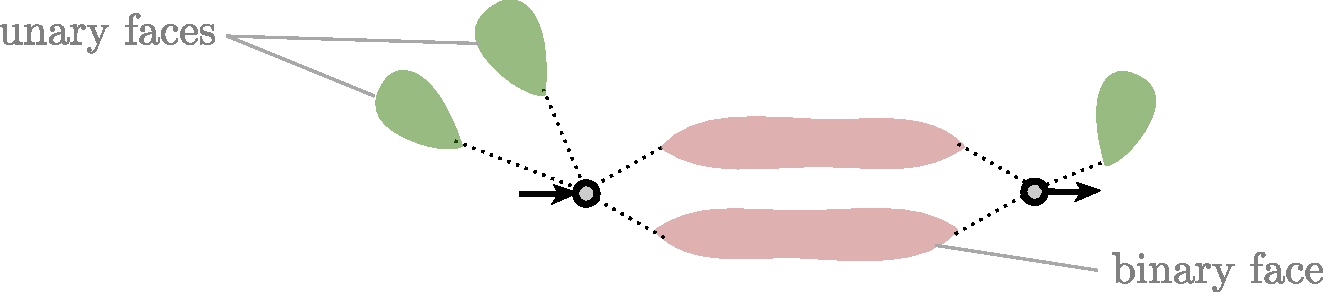
\includegraphics[scale=.4]{Pictures/unary-and-binary-faces}
\end{center}
\noindent We say that $G$ is \emph{pure} if  it has at least one face and  all it faces have the same arity as itself.  We say that $G$ is \emph{prime} if it has exactly one face, and \emph{composite} if it has at least two faces. 
\end{definition}


   \begin{remark} Pure graphs are connected and non-empty.  Not all graphs are pure.
   \end{remark}

   \begin{definition}[Type of a pure graph]
The \emph{type} of a pure graph is a pair specifying its arity and whether it is prime or composite. We say that a graph is \emph{series} if it is binary and prime, \emph{parallel} if it is binary and composite, \emph{domain} if it is unary and prime and \emph{test} if it is unary and composite. We denote by $\mathsf{s}, \mathsf{p}, \mathsf{d}$ and $\mathsf{t}$ the type series, parallel, domain and test respectively. Series, parallel domain and test graphs look like this:
   \begin{center}
   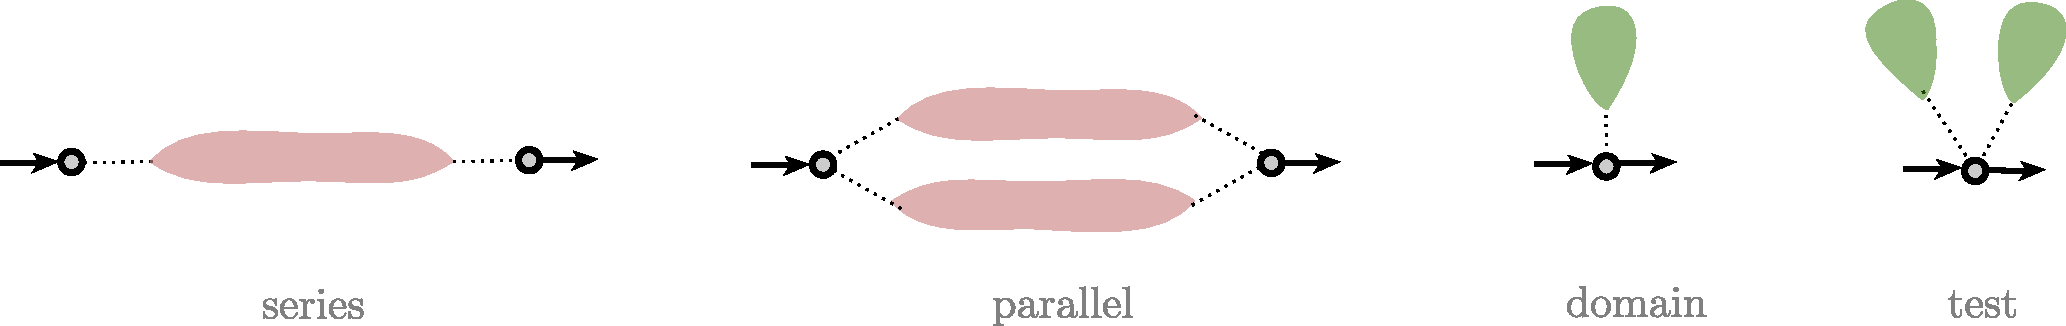
\includegraphics[scale=.4]{Pictures/spdt}
   \end{center}
   A graph language is (of type) \emph{series}, \emph{parallel}, \emph{domain} or \emph{test} if \textbf{all} its graphs have this type.  
   \end{definition}
   
   There is a canonical way to decompose pure graphs of type series, parallel and test. 
 \begin{proposition}[\cite{Damien}]
 Let $G$ be a pure graph. The graph $G$ has the following shape:
 $$\begin{array}{llll}
 G&:=&  P_0\cdot U_1 \cdot P_1 \dots U_n\cdot P_n & \qquad \qquad\text{ if $G$ is series,}\\[3pt]
 G&:=&  \ S_0\parallel  \dots \parallel S_n &  \qquad \qquad\text{ if $G$ is parallel,}\\[3pt]
 G&:=&  D_0\parallel  \dots \parallel D_n &  \qquad \qquad\text{ if $G$ is test,}\\
 \end{array}$$
 $P_j$ being parallel or atomic, $U_i$ unary, $S_i$ series and $D_i$ domain, for all $j\in[0,n], i\in[1,n]$.
\end{proposition}
Here is a picture illustrating this proposition:
\begin{center}
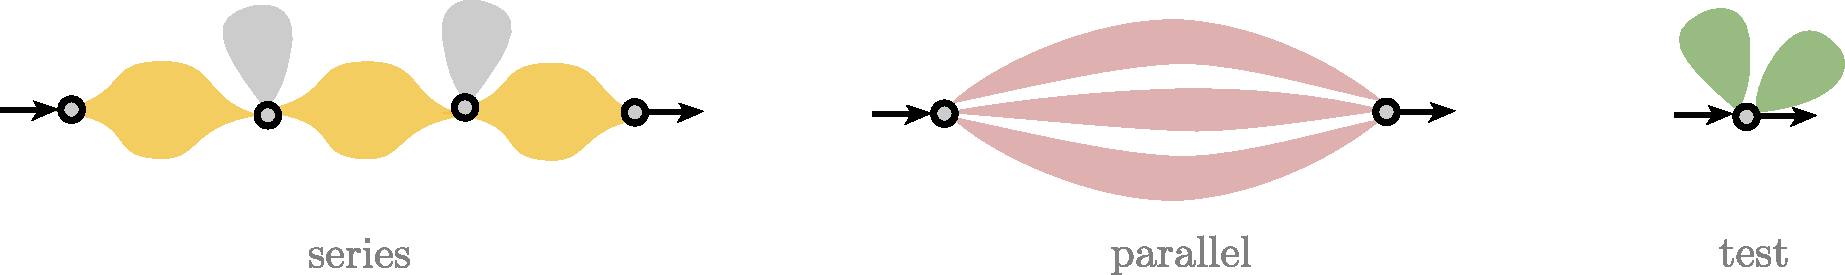
\includegraphics[scale=.35]{Pictures/spt}
\end{center}
\begin{definition}[Contexts]
A \emph{context} is a graph with a unique edge, labeled by a special letter, called its \emph{hole}.  If $C$ is a context whose hole is $h$ and $H$ a graph \textbf{with the same arity as $h$}, we define $C[H]$ as the graph obtained from the disjoint union of $C$ and $H$, by removing the edge $h$,  identifying the input of $h$ with the input of $H$, the output of $h$ with the output of $H$, and  by letting the interface of $C[H]$ to be that of $C$. 
Let $\mathbb{S}$ be a set of \emph{special (unary and binary) letters}, and let $n\geq 1$. An \emph{$n$-context}  is a graph such that $n$ of its edges, called \emph{holes}, are numbered from $1$ to $n$, and labeled by $n$ distinct special letters.  We call $1$-contexts simply \emph{contexts}.

Let $C$ be an $n$-context whose holes are $h_1\dots,h_n$ and let $H_1,\dots,H_n$ be graphs such that $h_i$ and the $H_i$ have the same arity, for all $i\in [1, n]$.  We define $C[H_1,\dots,H_n]$ as the graph obtained from the disjoint union of $C$ and $H_1,\dots, H_n$, by removing the holes of $G$, and for every $i\in[1,n]$  identifying the input of $h_i$ with the input of $H_i$, the output of $h_i$ with the output of $H_i$, and  by letting its interface to be that of $C$.\todo{do I use general contexts?}
\end{definition}

\begin{definition}[Islands and modules]  
An \emph{island} of a graph $G$ is a graph $H$ such that there is a context $C$ satisfying $G=C[H]$.  A \emph{module} is a island which is pure.  Two islands (or modules) of a graph are \emph{parallel} if they have the same interface. 

\noindent Since modules are pure, we can speak of series, parallel, domain and test modules  of a graph. 
\end{definition}

The following picture illustrates a unary and binary island of a graph.
\begin{center}
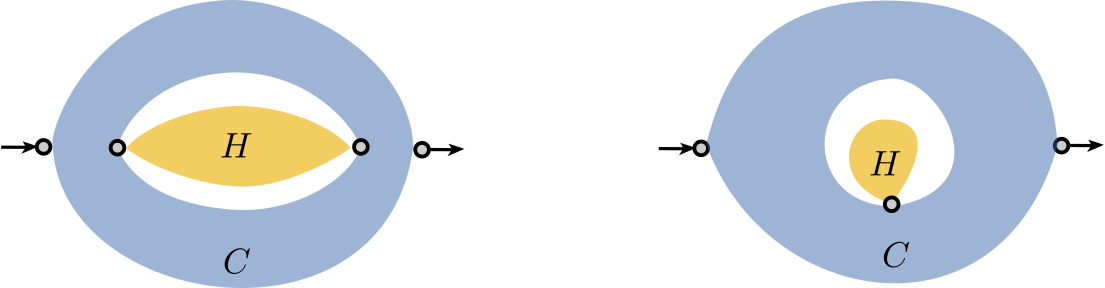
\includegraphics[scale=.35]{Pictures/island}
\end{center}
\begin{remark} Our notion of modules is different from the one usually used in graph theory, more precisely in the setting of \emph{modular decompositions}. %There, $X$ is a module if, for each vertex $v \not\in X$, either every member of $X$ is a non-neighbor of $v$ or every member of $X$ is a neighbor of $v$.
\end{remark}
 
 \begin{remark}
If $I$ is an interface in a graph $G$,  there is always an island of $G$ whose interface is $I$, the empty graph for example. This is not the case for modules.   
\end{remark}

\begin{remark}
The parallel composition of two islands of a graph $G$ with the same interface is also an island of $G$ with the same interface. Similarly, the parallel composition of two modules of a graph $G$ with the same interface is also a module of $G$ with the same interface. This justifies the following definition.
\end{remark}

\begin{definition}[Maximal islands and modules]
 Let $G$ be a graph and $I$ an interface in $G$.  The \emph{maximal island  at $I$} is the parallel composition of all the islands of $G$ whose interface is $I$, we denote it by $\mathsf{max}\text{-}\mathsf{island}_G(I)$. The \emph{maximal module at $I$} is the parallel composition of all the modules of $G$ whose interface is $I$, we denote it by $\mathsf{max}\text{-}\mathsf{module}_G(I)$.
\end{definition}
\begin{remark}
The maximal module at a given interface does not always exist.
\end{remark}

\begin{proposition}\label{prop:pure-modules-are-CMSO}
Being series, parallel, domain, test, an island, a module, a maximal island, a maximal module are $\CMSO$ definable properties. 
\end{proposition}
\begin{proof} We propose an equivalent definition for islands which is more convenient to express in $\CMSO$.
\begin{lemma}\label{lem:module} Let $G$ be a graph. A  subgraph $H$ of $G$ is an island iff no interface vertex of $G$ in an inner vertex of $H$ and there is no edge from an inner vertex of $H$ to a vertex of $G$ outside of $H$.
\end{lemma}
\begin{proof}
It is easy to see that if $H$ is an island, then it satisfies  these conditions.
Suppose that $H$ satisfies the conditions of the lemma. Let $C$ be the graph obtained from $G$ by removing all the edges and the inner vertices of $H$ and by adding a edge labeled by a special letter, with the same interface as $H$. It is easy to see that $C[H]$ is $G$.
\end{proof}
In $\CMSO$, we can express that a graph is not a maximal module: there is a module with the same interface, which is strictly bigger. Hence we can express maximality.

Since connectivity is expressible in $\CMSO$, we can express easily in $\CMSO$ that a subgraph is a face. We can also say if a a graph is series, by saying that it has a unique face, and this face is binary. We can proceed similarly to express that a graph is parallel,  domain, test and pure. Finally, we express that a graph is a module by saying that it is an island which is pure.    
\end{proof}

